% CIGL manuscript — LaTeX-ready draft (Phase 4H / v0.6).
% WRITING/PACKAGING ONLY. Do NOT compile a PDF without explicit reviewer authorization.
% Scientific claim is FIXED and BOUNDED (see ../cigl/CLAIMS_AUDIT.md): DGCNN static-adjacency backbone;
% graph/node posterior-KL proxy (NOT unbiased CMI); lambda_g = lambda_n = 0.010, lambda_edge = 0; two MI
% datasets; source-only DG; PARTIAL leakage reduction at source-task retention; no edge-CMI, no SOTA,
% no beyond-MI claim. Neutral article class on purpose — no conference template added in this phase.
\documentclass[11pt]{article}

\usepackage[utf8]{inputenc}
\usepackage[T1]{fontenc}
\usepackage{amsmath,amssymb}
\usepackage{booktabs}
\usepackage{graphicx}
\usepackage[numbers]{natbib}
\usepackage{hyperref}

\title{CIGL: Auditing and Reducing Label-Conditional Domain Leakage in EEG Graph
Representations under Source-Only Generalization}
\author{(authors omitted for anonymous draft)}
\date{Draft v0.6 / Phase 4H --- not for submission}

\begin{document}
\maketitle

\begin{abstract}
Cross-subject electroencephalography (EEG) decoders are confounded by subject- and session-specific
structure that a model can exploit instead of the task signal. We study this as \emph{label-conditional
domain leakage} in learned EEG graph representations: how much subject/domain identity a graph network's
graph-level and node-level features carry once the class label is fixed. We measure it with a
\emph{posterior-KL plug-in proxy} --- a conditional-domain probe scored against a retrained, within-label
permutation null --- and emphasize that this proxy is \emph{not} an unbiased conditional-mutual-information
(CMI) estimator. On a task-capable graph backbone (a DGCNN with a shared/static adjacency), we find the
graph and node representations carry significant such leakage. We then add a fixed \textbf{graph/node}
conditional-information regularizer (no edge term) and show, under \textbf{strict source-only} domain
generalization on two motor-imagery (MI) datasets, that it \textbf{partially but reproducibly reduces} this
leakage while meeting the pre-specified source-task retention criteria. The reduction is partial (the
regularized leakage still clears the null), the estimator is a proxy, the backbone is a single
static-adjacency graph network, and the evidence is two MI datasets --- we make no SOTA,
leakage-elimination, edge-CMI, cross-architecture, or beyond-MI claim. We also report the negative results
that shaped the method (a near-chance graph backbone and overfitting dynamic-edge designs), which justify
the bounded scope.
\end{abstract}

\section{Introduction}

EEG brain--computer interfaces must generalize across subjects, yet inter-subject variability is large and
a decoder can latch onto subject identity rather than the neural task. A growing line of work treats this
as a domain-generalization (DG) problem and as a \emph{shortcut/leakage} problem: features that separate
subjects, conditioned on the label, are a direct measure of how much the representation could be exploiting
domain identity. Graph neural networks are attractive for EEG because electrodes form a natural graph, and
they expose interpretable objects --- a graph-level readout, per-electrode node features, and (for some
designs) a learned adjacency. This makes them a good substrate for \emph{auditing} leakage at the graph and
node level.

Most leakage-control work either presumes a task-capable model or measures leakage without first confirming
that the backbone can learn the task at all; on EEG graph networks, we find neither holds for free. This
paper therefore makes a deliberately \textbf{bounded} contribution. We \emph{audit} label-conditional
domain leakage in a graph network's \texttt{graph\_z}/\texttt{node\_z} objects under a strict
no-target-label firewall; we then show --- through a methodology chain whose negative results are part of
the evidence --- that leakage control is only meaningful on a \emph{task-capable} graph backbone, which is
nontrivial to obtain; and we finally confirm that a single fixed graph/node conditional-information
regularizer reduces the audited leakage on two MI datasets while meeting a pre-registered source-task
retention gate. We do not claim state-of-the-art accuracy, leakage elimination, an unbiased CMI estimate,
an edge-level method, or generality beyond this backbone and these two MI datasets. The contributions are:

\begin{itemize}
  \item[\textbf{(C1)}] A \textbf{source-only audit} of label-conditional domain leakage in a graph
  network's \texttt{graph\_z}/\texttt{node\_z} objects: a posterior-KL plug-in proxy with a retrained
  within-label permutation null and a target-label firewall (we explicitly disclaim unbiased CMI).
  \item[\textbf{(C2)}] A \textbf{methodology chain, including its negative results}, showing that a
  \emph{task-capable} graph backbone is a prerequisite --- the original graph backbone is near-chance,
  dynamic-edge designs overfit, and a static-adjacency DGCNN is the one that learns the task.
  \item[\textbf{(C3)}] A \textbf{fixed-candidate, cross-dataset confirmation} that a graph/node
  conditional-information regularizer ($\lambda_g = \lambda_n = 0.010$, no edge term) partially and
  reproducibly reduces the audited leakage while meeting the pre-registered source-task retention gate on
  two MI datasets (the gate holds dataset-wide, with one BNCI2015\_001 fold missing the per-fold threshold).
  \item[\textbf{(C4)}] An explicit \textbf{negative-results $+$ limitations} account that bounds the claim
  (proxy not unbiased CMI; partial not full; graph/node only; one backbone; two MI datasets).
\end{itemize}

\section{Related Work}

We connect to four threads. (i) \textbf{EEG domain generalization / cross-subject MI}, especially the MOABB
benchmarking protocol~\citep{jayaram2018moabb}, from which our datasets and leave-one-subject-out (LOSO)
evaluation derive. (ii) \textbf{Graph EEG networks} --- DGCNN~\citep{song2018dgcnn},
RGNN~\citep{zhong2019rgnn}, and LGGNet~\citep{ding2021lggnet} --- which motivate graph/node/edge objects.
(iii) \textbf{Known-good convolutional MI decoders} --- EEGNet~\citep{lawhern2018eegnet} and
ShallowConvNet/DeepConvNet~\citep{schirrmeister2017deep} --- which we use only as sanity references for task
learnability. (iv) \textbf{Conditional-invariance / information-penalty} methods --- conditional
domain-invariant representations~\citep{li2018conditional}, classifier-based CMI / posterior-KL leakage
proxies~\citep{mukherjee2020ccmi}, and domain-adversarial or marginal-invariance baselines.

CIGL differs by (a) \emph{auditing} graph and node leakage explicitly with a permutation-null proxy before
regularizing, (b) operating strictly source-only with target labels evaluation-only, and (c) restricting to
a graph/node penalty on a task-capable static-adjacency backbone rather than claiming a general
edge/dynamic-graph method. A positioning grid and per-citation verification status are kept in
\texttt{../cigl/RELATED\_WORK\_MATRIX.md} and \texttt{../cigl/CITATION\_TODO\_QUEUE.md}.

% CMI-Trace P0.5 related-work correction (exact prose from paper/cmi_trace/MANUSCRIPT_INTEGRATION.md).
% arXiv IDs are cited inline as text (no \citep key added, because REFERENCES_DRAFT.bib lives outside
% paper/cigl_latex/ and this revision is scoped to that directory only).
{\sloppy
\paragraph{Concurrent subject-identity audits.}
Two concurrent audits of subject identity in EEG foundation models are complementary to ours but ask
different questions. \textbf{Lin, Wu, and Jung (arXiv:2606.06647)} study \emph{marginal} subject dominance
in frozen foundation-model features --- LEACE-based erasure, the spectral carrier of subject identity, and
the consistency of the task axis --- i.e.\ a geometry/erasure audit of the marginal subject signal.
\textbf{Tai (arXiv:2606.09189)} is a \emph{privacy / attribute-leakage} study auditing cross-encoder
attribute transfer (whether attributes leak across independently trained encoders), not a marginal
subject-variance audit. We therefore do \textbf{not} describe both as ``marginal subject-variance audits.''
Crucially, FMScope's cohort-conditioned \emph{frozen-feature} diagnostic (an oracle that fits the erasure
geometry on the whole cohort, including the held-out subject's features) and our strict source-only
\emph{unseen-subject deployment} ask different questions and \textbf{can both be correct}: cohort-conditioned
geometry can be erasable while the same axis is not identifiable, or removable, from source subjects alone
(P0.5 bridge, oracle vs source-only).\par}

\section{Method}

\paragraph{Backbone.} We use a DGCNN-style graph network with a single shared (static) learned adjacency and
a Chebyshev graph convolution over electrode nodes, exposing
$\texttt{forward\_graph}(x) \rightarrow (\text{logits}, \texttt{graph\_z}, \texttt{node\_z},
\texttt{edge\_logits})$. Because the adjacency is shared across samples, there is \textbf{no per-sample edge
object} ($\texttt{edge\_logits} = \texttt{None}$); CIGL as studied here is therefore \textbf{graph/node only}.
We adopt this backbone after an explicit search (Section~\ref{sec:analysis}): it is the graph-compatible
backbone we found that actually learns the task.

\paragraph{Leakage objects and proxy.} Let $Z_g$ be the graph readout and $Z_v$ the per-electrode node
features, $Y$ the class label, and $D$ the source-domain (subject) label. We quantify label-conditional
domain leakage with a \textbf{posterior-KL plug-in proxy}:
\begin{align}
R_g &= \mathbb{E}\!\left[ \mathrm{KL}\!\left( q_g(D \mid Z_g, Y) \,\Vert\, \pi_y(D) \right) \right], &
R_n &= \frac{1}{C} \sum_{v} \mathbb{E}\!\left[ \mathrm{KL}\!\left( q_n(D \mid Z_v, v, Y) \,\Vert\,
\pi_y(D) \right) \right],
\end{align}
where $q_g$/$q_n$ are conditional-domain posterior heads, $\pi_y(D)$ the within-label domain prior, and $C$
the number of electrodes. We stress that $R_g$/$R_n$ are a \textbf{proxy}, not an unbiased CMI estimator.

\paragraph{Regularizer.} CIGL trains the backbone with $\mathcal{L} = \mathcal{L}_{\mathrm{CE}} +
\lambda_g R_g + \lambda_n R_n$ (no edge term), using the established two-step scheme: Step~A fits the
posterior heads on detached features; Step~B penalizes the encoder. Throughout the confirmation we use a
single \textbf{fixed} weight $\lambda_g = \lambda_n = 0.010$ ($\lambda_{\mathrm{edge}} = 0$). The pipeline is
sketched in Figure~\ref{fig:pipeline}.

% Figure 2 Panel A/B (see paper/cmi_trace/MANUSCRIPT_INTEGRATION.md, P0.3): the study-architecture / audit
% pipeline is split into TWO panels joined by a DASHED bridge -- Panel A = same-backbone objective audit
% (the P0.1/P0.2 contribution; CIGL's static-adjacency DGCNN + posterior-KL is the Encoder-CMI objective in
% this panel), Panel B = complementary representation-level (EEGNet/TSMNet geometry + deployment) extension.
% The objective comparison (P0.1) is still producing (jobs 896396/896397); this figure shows the STUDY
% DESIGN, not results. Schematic only; no result numbers are asserted here.
\begin{figure}[t]
  \centering
  \fbox{\parbox{0.92\linewidth}{\centering\small\textbf{[F2 --- study architecture, schematic, DRAFT]}\\[3pt]
  \textbf{Panel A --- same-backbone objective audit.}\\[1pt]
  ERM / CORAL / C-CORAL / IRMv1 / V-REx / conditional-adversarial / Encoder-CMI
  (\emph{all} on the \textbf{same} static-adjacency DGCNN adapter, source-only LOSO, cloned init; CIGL's
  \texttt{graph\_z}/\texttt{node\_z} posterior-KL, $\lambda=0.010$, is the Encoder-CMI objective)
  $\rightarrow$ marginal $+$ class-conditional moment gaps
  $\rightarrow$ graph/node encoder-CMI $+$ retrained within-label permutation null
  $\rightarrow$ per-domain risk variance $+$ IRMv1 diagnostic (post hoc)
  $\rightarrow$ exact original-head reliance $R_{\mathrm{rel}}(k{=}2)$ $+$ same-rank random control
  $\rightarrow$ target balanced accuracy. \\[4pt]
  $-\;-\;-\;-\;-$\; \emph{dashed bridge: complementary representation-level extension} \;$-\;-\;-\;-\;-$ \\[4pt]
  \textbf{Panel B --- complementary geometry \& deployment extension.}\\[1pt]
  EEGNet / TSMNet frozen representations
  $\rightarrow$ TOS / LEACE / RLACE / INLP / random-$k$
  $\rightarrow$ nonlinear subject residual
  $\rightarrow$ capacity factorial
  $\rightarrow$ source-fitted target deployment. \\[2pt]
  \textit{Draft vector asset: \texttt{figures/fig1\_pipeline\_draft.svg} (to be regenerated as two panels).}}}
  \caption{Study architecture (schematic draft). \textbf{Panel A} is the same-backbone objective audit: every
  objective is trained on the \emph{same} static-adjacency DGCNN adapter under the same source-only LOSO
  protocol and passed through one shared audit; CIGL's graph/node posterior-KL regularizer is the
  Encoder-CMI objective within this panel. \textbf{Panel B}, joined only by a \emph{dashed} bridge, is a
  \emph{complementary representation-level extension} on EEGNet/TSMNet frozen features (geometry probes and
  source-fitted target deployment); it is \textbf{not} claimed that every Panel-A objective underwent every
  TOS / deployment test. The posterior-KL terms are a proxy, not an unbiased CMI estimator.}
  \label{fig:pipeline}
\end{figure}

\paragraph{Audit.} To judge significance we re-fit fresh held-out conditional-domain probes on frozen
features and compare to a \textbf{retrained, within-label permutation null} (permuting $D$ within label on
the probe-training split only, preserving the within-label prior);
$\texttt{clears\_null} = (\texttt{kl\_mean} > \texttt{permutation\_mean})\;\wedge\;
(\texttt{permutation\_p} \le 0.05)$. The audit is the same proxy used as a measurement, never inverted into
an information-theoretic guarantee. Figure~\ref{fig:audit} shows the audit against the null on the
development fold.

\begin{figure}[t]
  \centering
  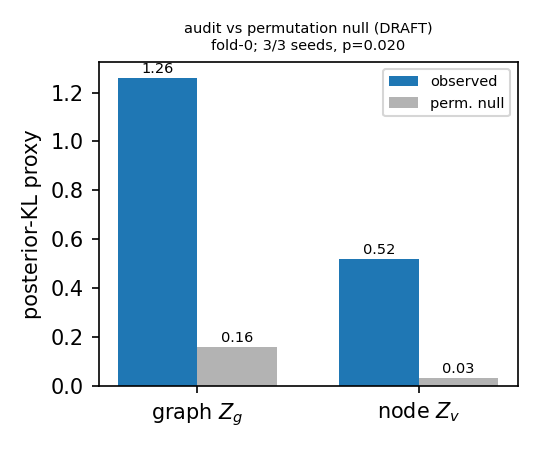
\includegraphics[width=0.5\linewidth]{figures/fig3_audit_null_draft.png}
  \caption{\textbf{[DRAFT, from data]} Source-only leakage audit on BNCI2014\_001 fold-0: observed
  posterior-KL proxy vs the retrained within-label permutation null for the graph and node objects (clears
  the null in 3/3 seeds, $p=0.020$). Values from the development-fold audit; not an unbiased CMI estimate.}
  \label{fig:audit}
\end{figure}

% CMI-Trace P1.5 notation clarification: distinct symbols for the in-loop training regularizer vs the
% held-out audit estimate; "cross-fitted neural posterior plug-in estimate" (no bound proved); raw nats +
% secondary normalized readout; finite-critic underfitting can UNDER-report leakage.
\paragraph{Notation and the training/audit distinction.} We keep the \emph{in-loop training regularizer}
$\mathcal{L}^{\mathrm{CMI}}_{\mathrm{train}} = \lambda_g R_g + \lambda_n R_n$ (computed on the training split
--- on detached features in Step~A and as the encoder penalty in Step~B) notationally distinct from the
\emph{held-out audit estimate} $\hat{I}_{\mathrm{audit}}$, obtained by re-fitting fresh conditional-domain
probes on frozen held-out features. $\hat{I}_{\mathrm{audit}}$ is a \textbf{cross-fitted neural posterior
plug-in estimate}; no information-theoretic bound is proved for it. The two quantities share the posterior-KL
form but are computed on disjoint data and are \emph{not} interchangeable. Because a finite-capacity critic
can \emph{under}-report leakage, $\hat{I}_{\mathrm{audit}}$ is a lower-confidence proxy, never a guarantee. We
report $\hat{I}_{\mathrm{audit}}$ in raw nats, with a secondary normalized readout
$\hat{I}_{\mathrm{audit}} / \hat{H}(D \mid Y)$ used only for cross-dataset comparison.

\section{Experimental Protocol}

We evaluate under \textbf{strict source-only DG}: a leave-one-subject-out (LOSO) target is excluded from
training and from the source probe used for selection; \textbf{target labels are evaluation-only} and never
used for training, early stopping, normalization, model/config selection, confirmation-label choice, probe
fitting, or the audit. We use two MI datasets: \textbf{BNCI2014\_001}~\citep{tangermann2012review,
brunner2008graz2a} (4-class, chance $0.25$) and \textbf{BNCI2015\_001}~\citep{faller2012autocalibration}
(binary right\_hand vs.\ feet, chance $0.50$; loaded via the \texttt{MotorImagery} paradigm because it is
not left/right-hand). Both use MOABB preprocessing~\citep{jayaram2018moabb} at $128$~Hz, a $0.5$--$3.5$~s
window, and per-trial $z$-scoring; data come from a read-only datalake. The candidate
$\lambda_g = \lambda_n = 0.010$ was selected once on a single development fold (BNCI2014\_001 fold-0) and
then \textbf{frozen}; all subsequent runs are fixed-candidate confirmations with no $\lambda$ search.
Table~1 (\texttt{tables/table1\_method\_protocol.tex}) summarizes the method/config/protocol.

\section{Results}
\label{sec:results}

\paragraph{Leakage exists on a task-capable backbone.} On the DGCNN backbone (BNCI2014\_001 fold-0), the
graph and node objects carry strong, significant, and spatially stable leakage: the graph proxy is
$\approx 8\times$ and the node proxy $\approx 15\times$ the permutation mean, clearing the null in $3/3$
seeds, with a node-leakage map highly reproducible across seeds (mean pairwise correlation $\approx 0.945$).
This is the first such audit on a backbone that \emph{also} learns the task (Table~\ref{tab:leakage_audit}).

% Table 2 — DGCNN leakage audit (CIGL_25, BNCI2014_001 fold-0). Draft; values from RESULTS_TABLES_DRAFT.md (T2).
\begin{table}[t]
\centering
\caption{Source-only leakage audit on the DGCNN backbone (BNCI2014\_001 fold-0). The proxy is compared to a
retrained within-label permutation null; \texttt{clears} = significant in 3/3 seeds. Edge is skipped
(static adjacency, \texttt{edge\_logits=None}).}
\label{tab:leakage_audit}
\small
\begin{tabular}{lcccc}
\toprule
Object & kl\_mean & perm\_mean & $p$ & clears (seeds) \\
\midrule
graph $Z_g$ & $\approx 1.26$ ($\approx 8\times$ perm)  & $\approx 0.16$  & 0.020 & 3/3 \\
node $Z_v$  & $\approx 0.52$ ($\approx 15\times$ perm) & $\approx 0.034$ & 0.020 & 3/3 \\
\bottomrule
\end{tabular}

\vspace{2pt}
\footnotesize Node-leakage map stable across seeds (mean pairwise corr.\ $\approx 0.945 \gg$ null q95 $\approx 0.20$).
\end{table}


\paragraph{Fixed regularizer reduces leakage at task retention --- two datasets.} On \textbf{BNCI2014\_001}
(primary folds 1--8; fold-0 is the development fold and is excluded), the fixed \texttt{graph\_node\_010}
passes all four source-only criteria in every primary fold while meeting the source-task retention gate
(absolute drop $\le 0.02$); graph and node proxy reductions and their fold-level bootstrap confidence
intervals are in Table~\ref{tab:bnci2014}. On \textbf{BNCI2015\_001} (all 12 LOSO folds), the same fixed candidate is
ERM-adequate, leakage-bearing, and leakage-reducing in $12/12$ folds, meets the retention gate in $11/12$
folds (one fold misses the per-fold threshold; the dataset-level gate passes), and holds the
evaluation-only target guardrail in $12/12$ folds, yielding
$\texttt{confirmed\_with\_target\_guardrail} = \texttt{true}$; reductions and CIs are in
Table~\ref{tab:bnci2015}. Figure~\ref{fig:retention} plots every fold's reduction against its source-task
retention.

% Table 3 — BNCI2014_001 confirmation (CIGL_29; primary folds 1-8; fold-0 = dev, excluded).
% Draft; means/ranges from RESULTS_TABLES_DRAFT.md (T3); 95% CIs from STATISTICAL_SUMMARY_DRAFT.md
% (fold-level bootstrap, seed 0, 10000 resamples, percentile).
\begin{table}[t]
\centering
\caption{BNCI2014\_001 confirmation of the fixed \texttt{graph\_node\_010} (primary folds 1--8; fold-0 is
the development fold, excluded). bAcc = balanced accuracy (chance 0.25); KL reduction = $(\mathrm{ERM}-
\mathrm{reg})/\mathrm{ERM}$ of the posterior-KL proxy. 95\% CIs are fold-level bootstrap. ``retain'' = source
drop $\le 0.02$. Edge skipped.}
\label{tab:bnci2014}
\small
\begin{tabular}{lc}
\toprule
Quantity & Value \\
\midrule
fold group / $n_{\mathrm{folds}}$        & primary folds 1--8 / 8 \\
ERM source bAcc (mean [range])           & 0.484 [0.457, 0.508] \\
reg source bAcc (mean, 95\% CI)          & 0.488 [0.471, 0.505] \\
source retention (drop $\le 0.02$)       & 8/8 \\
graph KL reduction (mean, 95\% CI; range)& 44.0\% [39.5, 49.0]; 35--58\% \\
node KL reduction (mean, 95\% CI; range) & 36.9\% [33.6, 40.3]; 31--45\% \\
ERM leakage clears null / reg reduces $\ge$30\% & 8/8 / 8/8 \\
target guardrail (drop $\le 0.05$)       & 8/8 \\
reg leakage still clears null            & every fold (partial, not elimination) \\
edge status / decision                   & skipped / \textbf{A} \\
\bottomrule
\end{tabular}
\end{table}

% Table 4 — BNCI2015_001 confirmation (CIGL_31; all 12 LOSO folds).
% Draft; means/ranges from RESULTS_TABLES_DRAFT.md (T4); 95% CIs from STATISTICAL_SUMMARY_DRAFT.md
% (fold-level bootstrap, seed 0, 10000 resamples, percentile).
\begin{table}[t]
\centering
\caption{BNCI2015\_001 confirmation of the same fixed \texttt{graph\_node\_010} (all 12 LOSO folds). bAcc
chance 0.50. 95\% CIs are fold-level bootstrap. One fold (fold9, $+0.024$) misses the per-fold retention
threshold while the dataset-level gate passes. Edge skipped.}
\label{tab:bnci2015}
\small
\begin{tabular}{lc}
\toprule
Quantity & Value \\
\midrule
fold group / $n_{\mathrm{folds}}$        & all LOSO folds / 12 \\
ERM source bAcc (mean [range])           & 0.706 [0.682, 0.734] \\
reg source bAcc (mean, 95\% CI)          & 0.700 [0.693, 0.707] \\
source retention (drop $\le 0.02$)       & 11/12 (fold9 $+0.024$) \\
graph KL reduction (mean, 95\% CI; range)& 66.2\% [60.6, 71.0]; 43--77\% \\
node KL reduction (mean, 95\% CI; range) & 51.9\% [47.8, 55.6]; 37--61\% \\
ERM adequacy / leakage / reg reduces $\ge$30\% & 12/12 / 12/12 / 12/12 \\
target guardrail (drop $\le 0.05$)       & 12/12 \\
reg leakage still clears null            & every fold (partial, not elimination) \\
edge status / decision                   & skipped / \textbf{A} (\texttt{confirmed\_with\_target\_guardrail=true}) \\
\bottomrule
\end{tabular}
\end{table}


\begin{figure}[t]
  \centering
  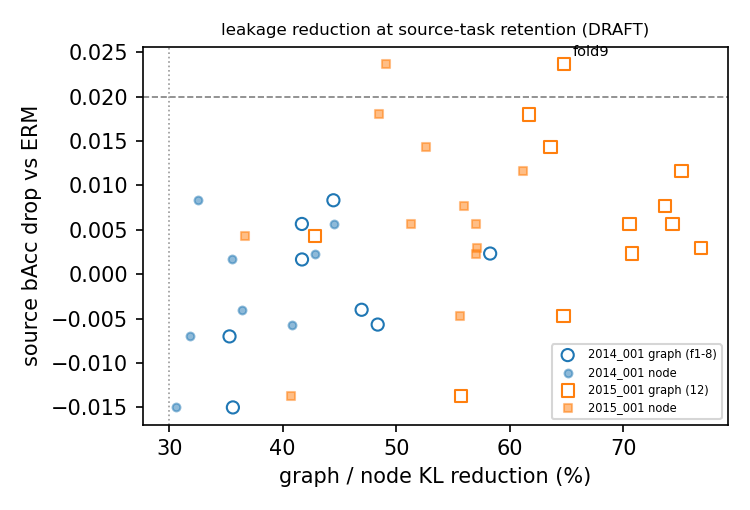
\includegraphics[width=0.62\linewidth]{figures/fig2_reduction_vs_retention_draft.png}
  \caption{\textbf{[DRAFT, from data]} Per-fold graph/node KL reduction (\%) vs source bAcc drop relative to
  ERM, for BNCI2014\_001 (folds 1--8) and BNCI2015\_001 (12 folds). The $y$-axis is a \emph{retention} axis:
  near-zero drop means the task is retained, not improved. The dashed line is the retention gate
  ($\text{drop}\le 0.02$); the single BNCI2015\_001 point above it (fold9, $+0.024$) is annotated. Values
  from the per-fold confirmation logs.}
  \label{fig:retention}
\end{figure}

\paragraph{Partial, not total.} In every confirmation fold the \emph{regularized} leakage still clears the
null --- CIGL reduces the proxy substantially (see Tables~\ref{tab:bnci2014}--\ref{tab:bnci2015}) but does
not eliminate the leakage. We report reduction, not removal.

\section{Analysis and Negative Results}
\label{sec:analysis}

The negative results are part of the contribution; they justify the bounded scope.

\begin{itemize}
  \item[(i)] \textbf{The original graph backbone fails the task.} A GraphCMINet-style network is near-chance
  under strict source-only training and is not repairable by small training tweaks, so its (strong,
  controllable) leakage cannot support a task-vs-leakage tradeoff.
  \item[(ii)] \textbf{The protocol is learnable.} Known-good convolutional decoders
  (EEGNet/ShallowConvNet/DeepConvNet) and a DGCNN all clear a source-accuracy floor on the same fold,
  showing the bottleneck was the specific graph backbone, not the data/protocol.
  \item[(iii)] \textbf{Dynamic-edge designs overfit.} The tested dynamic-adjacency backbones overfit
  strongly (train $\approx 1.0$, source $\approx$ chance) regardless of temporal stem, and carry leakage;
  this is consistent with a per-sample adjacency $A(x)$ acting as a subject-fingerprint channel, but these
  experiments do \textbf{not} causally isolate $A(x)$ as the only source of memorization. Either way,
  \textbf{dynamic-edge CIGL is unsupported here and edge-CMI is out of scope}.
\end{itemize}

The static-adjacency DGCNN is the only graph-compatible backbone that both learns the task and exposes
usable graph/node objects, which is why CIGL is framed as graph/node only on this backbone. Table~5
summarizes the negative results, and Figure~F4 shows the decision flow that fixed the scope.

\section{Limitations}

\begin{enumerate}
  \item The leakage metric is a \textbf{posterior-KL proxy}, not an unbiased CMI estimator; it can over- or
  under-state true CMI, so we frame it as an audit/penalty, not a guarantee.
  \item Control is \textbf{partial} --- the regularized leakage still clears the null.
  \item Evidence is \textbf{two MI datasets}; we make no beyond-MI or universal claim.
  \item Results are for \textbf{one backbone} (DGCNN static adjacency); no cross-architecture claim.
  \item A \textbf{single fixed} $\lambda$ ($0.010$) was confirmed; we ran no $\lambda$-grid and make no
  $\lambda$-robustness claim.
  \item The candidate was selected on a development fold before freezing; we report this and exclude that
  fold from the primary aggregate.
  \item Baselines are modest (BNCI2014\_001 ERM $\approx 0.46$; BNCI2015\_001 ERM $\approx 0.70$) --- this is
  a leakage-reduction-at-retention result, not an accuracy record.
  \item \textbf{No edge object} (static adjacency); edge/dynamic-graph leakage control is future work.
\end{enumerate}

\section{Conclusion}

We presented CIGL, a source-only audit and graph/node regularizer for label-conditional domain leakage in
EEG graph representations. On a task-capable static-adjacency DGCNN backbone, the audited graph/node leakage
is significant, and a fixed graph/node conditional-information regularizer partially and reproducibly
reduces it while meeting the pre-specified source-task retention criteria on two MI datasets. The
contribution is a bounded, honestly-scoped measurement$\rightarrow$control result, accompanied by the
negative results that shaped it. Future work includes constrained dynamic-edge backbones that generalize (to
enable an edge-level audit), additional datasets and paradigms, and tighter estimators than the posterior-KL
proxy.


\bibliographystyle{plainnat}
\bibliography{../cigl/REFERENCES_DRAFT}

\end{document}
